\newcommand\SelectionFlow{
    \begin{tikzpicture}
        \node (steps) {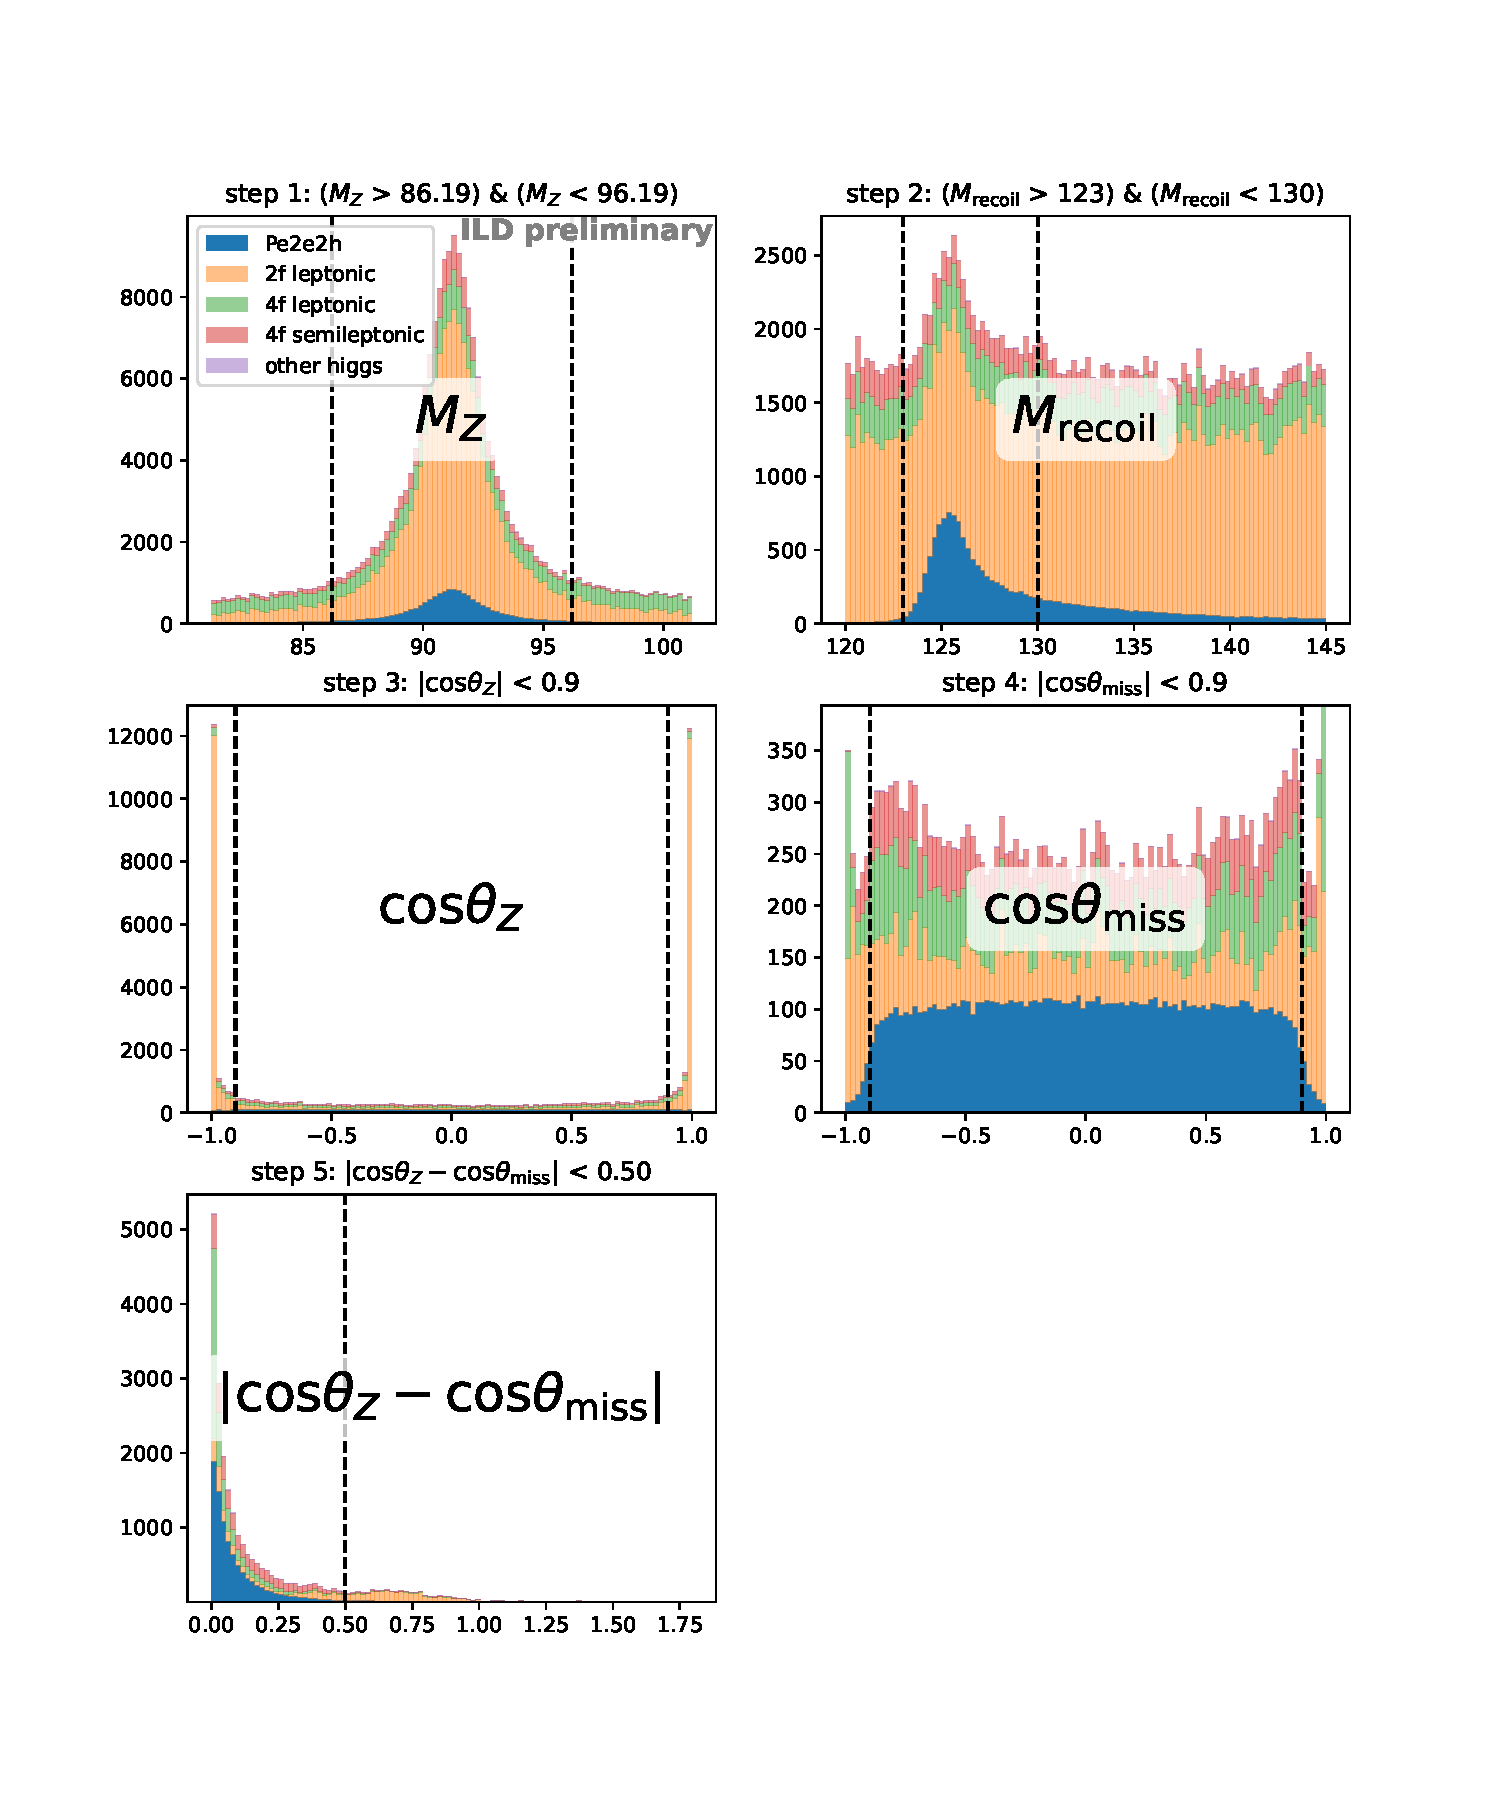
\includegraphics[width=0.9\textwidth]{presel_e2e2_5}};
        \node[anchor=south east] at (steps.south east) {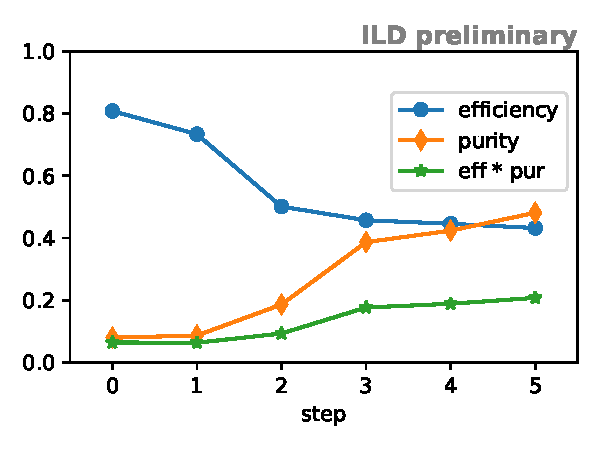
\includegraphics[width=0.45\textwidth]{presel_e2e2_eff_5}};
    \end{tikzpicture}
}

\begin{block}{1. Event selection}
    Solely information from recoiling Z boson is used: \\
    Independent of Higgs decay. \\
    Currently only with $Z \rightarrow \mu^+ \mu^-$, $Z \rightarrow e^+ e^-$ \\
    Higgsstrahlung events as signal channels.
\begin{columns}
\begin{column}{.5\textwidth}
    \begin{figure}
        \centering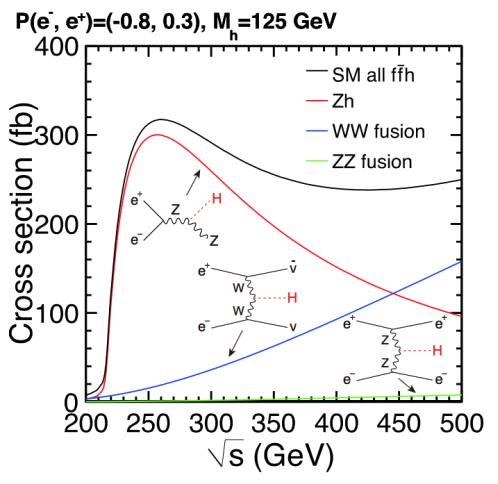
\includegraphics[width=0.8\textwidth]{IGP_xsec_h_ILC_left}
    \end{figure}
    \begin{itemize}
        \item Golden channels due to recoil mass method,
            $M_{\mathrm{recoil}}^2 = s + M_Z^2 - 2\sqrt{s} \cdot E_Z$.
        \item IsolatedLeptonTagger:
            Lepton pair with same type and opposite charge.
    \end{itemize}
\end{column}
\begin{column}{.5\textwidth}
    \begin{itemize}
        \item Final state radiation:
            Add photons with $\mathrm{cos}\theta_{l\gamma} > 0.99$.
        \item Selection cuts shown on the right.
    \end{itemize}
    \SelectionFlow
\end{column}
\end{columns}
\end{block}
